% ======================================================================
\section{Introduction}
\label{sec:intro}

\begin{figure}[t]
  \centering
  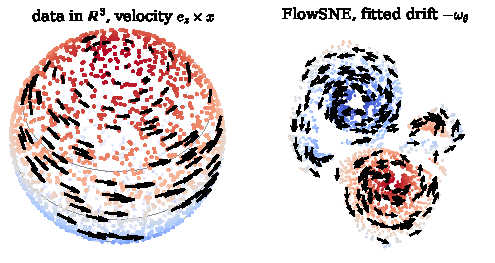
\includegraphics[width=\columnwidth]{figures/teaser_sphere.pdf}
  \caption{\emph{Left:} points on a sphere with a rotation velocity
  $e_z\times x$, coloured by height (red north, blue south).
  \emph{Right:} the 2-D FlowSNE embedding (row-stochastic input), fitted
  jointly with a drift field (arrows), same colours. The map tears the
  sphere along the equator; each hemisphere becomes a vortex centred on the
  image of its pole, where the true speed vanishes.}
  \label{fig:teaser}
\end{figure}

Neighbour embeddings are the standard way to look at high-dimensional
data. SNE, t-SNE and UMAP
\citep{hinton2002sne,vandermaaten2008tsne,mcinnes2018umap} turn pairwise
costs into an affinity matrix and fit a low-dimensional layout whose own
affinities match it. Their costs are symmetric: the affinity of $x_j$
seen from $x_i$ is built from the same number as that of $x_i$ seen
from $x_j$.

Many datasets, however, come with a \emph{direction} at each sample. In
single-cell transcriptomics, \emph{RNA velocity} estimates, for every
cell, where its gene expression is heading in the next hours
\citep{lamanno2018rna,bergen2020generalizing}: each data point comes with
a velocity vector in the same space. In a transformer, each layer adds an
update to the residual stream of every token. A flow-matching model
carries a velocity field by construction. A symmetric cost cannot express
that moving \emph{with} such a field is easier than moving against it,
so neighbour embeddings discard the direction. The common workaround
draws arrows afterwards. scVelo \citep{bergen2020generalizing}, the
standard tool in single-cell analysis, first fits a symmetric embedding,
then for each cell compares its velocity with the directions to its
neighbours in the data space, and draws an arrow towards the neighbours
the velocity points to, at their positions in the layout. The arrow
depends on the layout and on its neighbourhood graph, can only point
towards neighbours the symmetric map placed nearby, and may show a
direction the data do not support \citep{bergen2021rna}. The direction
is painted onto the map; it did not shape it.

The simplest direction-dependent geometry is a \emph{Randers} metric
\citep{randers1941asymmetrical,bao2000introduction}, a Euclidean norm
tilted by a drift field $\omega$ with $\|\omega\|<1$:
\begin{equation}
  F_x(v)=\|v\|+\omega(x)^\top v .
  \label{eq:randers}
\end{equation}
Moving along $\omega$ costs $1+\|\omega\|$ per unit length, moving
against it $1-\|\omega\|$. Plugging a Randers distance into the
entropic affinities of SNE seems straightforward, but raises three
questions. The distance is an infimum over paths with no closed form
when $\omega$ varies, so it must be approximated. Affinities are
normalised, by rows (SNE) or by Sinkhorn balancing (SNEkhorn,
\citealt{vanassel2023snekhorn}), and a normalisation rescales rows and
columns, which can absorb part of the asymmetry. Finally, the embedding
kernel must be able to express the direction it is asked to match.

\paragraph{Contributions.}
We introduce \emph{FlowSNE}, a neighbour embedding for data with
velocities (\cref{fig:teaser}), and answer these three questions.
\begin{itemize}
  \item \textbf{Randers affinities (\cref{sec:randers}).} Two closed-form
    approximations of the Randers distance built from the velocities at
    the endpoints only, with error $O(r^2)$ and $O(r^3)$ at distance
    $r$ (\cref{prop:approx}), define a perplexity-calibrated entropic
    affinity.
  \item \textbf{What normalisation keeps (\cref{sec:gauge}).} A
    Sinkhorn-balanced affinity is determined by its cost modulo
    separable functions (\cref{thm:identifiability}). It therefore sees
    the circulation of a drift and not its gradient part, which a
    row-stochastic affinity keeps as a tilt of its column marginal. A
    uniform drift is invisible to a balanced affinity.
  \item \textbf{FlowSNE (\cref{sec:flowsne}).} The embedding kernel is a
    Student kernel on a Randers cost whose drift is a small neural network
    fitted jointly with the layout. The same gauge argument tells which
    part of this drift the loss can reward.
  \item \textbf{Implementation (\cref{sec:implementation}).} A
    TorchDR implementation with KeOps lazy tensors computes both costs
    in $O(n)$ memory and fits $10^5$ points on one GPU.
  \item \textbf{Experiments (\cref{sec:exp}).} On synthetic flows,
    clean or noisy and high-dimensional, FlowSNE recovers circulation,
    which embeddings with a constant Finsler drift cannot represent, and
    matches them in direction on gradient flows. On single-cell data the
    two normalisations behave as the theory predicts: on a
    differentiation process the row-stochastic input keeps the signal,
    while on the cell cycle, where an independent measurement of each
    cell's phase gives a ground truth, the balanced input isolates the
    circulation (0.68 against 0.39 for projected arrows) and the
    row-stochastic one fits the density instead. On GPT-2's residual
    stream, FlowSNE orients the rings that calendar tokens form.
\end{itemize}
